\subsection{Cholesky decomposition}

\begin{definition}
    $B \in \mathbb{R}^{n \times n}$ is positive definite if and only if:
    \begin{enumerate}
        \item {
            All eigenvalues are greater than 0.
        }
        \item {
            $v \cdot Bv > 0$ when $v \ne 0$.

            $v \cdot Bv = 0 \Longleftrightarrow v = 0$.
        }
    \end{enumerate}
\end{definition}

\begin{statement}
    When $B$ is symmetric and real, then all of the eigenvalues of it are real numbers.
\end{statement}

\begin{definition}[Cholesky decomposition]
    When $A \in \mathbb{R}^{n \times n}$ is symmetric and positive definite,
    then $A$ can be decomposed in the following form:
    \[ A = LDL^\intercal \]
    where:
    \begin{itemize}
        \item {
            $L$ is lower triangular, $a_{ii} = 1$, $i = 1, \dots, n$.
        }
        \item {
            $D$ is diagonal matrix with positive entries
        }
        \item {
            Because $D$ has only positive entries, we can we can 
            take the "square root" of it, i.e. find $\tilde{D}$, such that
            $D = \tilde{D} \tilde{D}$.
            So,
            \[ A = L D L^\intercal = (L\tilde{D}) (\tilde{D} L^T) = \tilde{L} \tilde{L}^\intercal \]
            Here $\tilde{D} = D$ as $D$ is diagonal.
        }
    \end{itemize}
\end{definition}

With such a decomposition, we can solve $Ax = b$ as
$Ax = \tilde{L} \tilde{L}^\intercal x = b$, where
$\tilde{L}$ is lower-triangular and $\tilde{L}^\intercal$ is upper-triangular.

The advantage from LU decomp is that we only need to save one matrix,
and forward substitution of the same kind will be carried out twice (so the matrix
will already be in cache).

The complexity if $\mathcal{O}(n^3)$, but compared to LU approximately half the operations
are needed.

How to compute $\widetilde{L}$? Let's suppose
\[
    \tilde{L} = \begin{bmatrix}
        l_{11} & 0 & \dots & 0\\
        l_{21}  & l_{22} & \dots & 0\\
        \vdots & \vdots & \ddots & \ddots\\
        l_{n1} & \dots & \dots & l_{nn}
    \end{bmatrix}
\] 
Then
\[
    \begin{bmatrix}
        a_{11} & \dots & a_{1n}\\
        \vdots & \ddots & \vdots\\
        a_{n1} & \dots & a_{nn}
    \end{bmatrix} =
    \begin{bmatrix}
        l_{11} & \dots & 0\\
        \vdots & \ddots & \vdots\\
        l_{n1} & \dots & l_{nn}
    \end{bmatrix} \cdot
    \begin{bmatrix}
        l_{11} & \dots & l_{n1}\\
        \vdots & \ddots & \vdots\\
        0 & \dots & l_{nn}
    \end{bmatrix}
\]
Then it follows by the formula of matrix multiplications:
\[ a_{ij} = \sum_{k=1}^n l_{ik} l_{jk} \]
Since a lot of entries in $\tilde{L}$ are zeros, actually
\[ a_{ij} = \sum_{k = 1}^j l_{ik} l_{jk},\ i \ge j \]
We only write such equations for $i \ge j$, as we have a symmetrical matrix
on the left hand side.

Now, for $i = j$:
\[
    a_{ii} = \sum_{k=1}^{i} l_{ik} l_{ik} = \sum_{k=1}^i (l_{ik})^2
    \Longleftrightarrow l_{ii} = \sqrt{a_{ii} - \sum_{k=1}^{i-1} (l_{ik})^2}
\]
Here $l_{ii}$ is non-negative, as in $L$ the diagonal elements are 1,
and $\tilde{L} = L \cdot \sqrt{D}$, which doesn't change the sign of the diagonal elements.

For $i > j$: \[ a_{ij} = \sum_{k=0}^j l_{ik} l_{jk} \]
and so:
\[ l_{ij} = \frac{1}{l_{jj}} \Bigl(a_{ij} - \sum_{k=1}^{j-1} l_{ik} l_{jk}\Bigr) \]
Finally $i < j: l_{ij} = 0$ as we have an lower triangular matrix.

This means we can compute entries of $\tilde{L}$ columnwise.

When does the algorithm fail? If we take the square root of a negative number
at some point, that means that the matrix was non-positive-definite.

\textbf{Algorithm:}\\
For $i=1 \dots n$:\\
\hspace*{0.5cm}For $j = 1 \dots i - 1$ (here $i > j$)\\
\hspace*{1cm} $y = a(i, j)$\\
\hspace*{1cm} For $k = 1 \dots j - 1$:\\
\hspace*{1.5cm} $y = y - l(i, k) \cdot l(j, k)$\\
\hspace*{1cm} end for\\
\hspace*{1cm} $l(i, j) = \frac{y}{l(j, j)}$\\
\hspace*{0.5cm} end for\\
\hspace*{0.5cm} $y = a(i, j)$ (here $i = j$)\\
\hspace*{0.5cm} For $k = 1 \dots i - 1$:\\
\hspace*{1cm} $y = y - l(i, k) \cdot l(i, k)$\\
\hspace*{0.5cm} end for\\
\hspace*{0.5cm} if $(y \le 0)$ exit (no solution)\\
\hspace*{0.5cm} else $l(i, j) = \sqrt{y}$\\
end for

The time complexity is $\mathcal{O}(n^3)$.

\begin{example}
    \[ 
        A = \begin{bmatrix}
            1 & 1 & 1\\
            1 & 2 & 3\\
            1 & 3 & 6
        \end{bmatrix}
    \]
    Compute $\tilde{L} \tilde{L}^\intercal = A$.
    Columnwise:
    \begin{align*}
        &
        l_{11} = \sqrt{a_{11}} = 1
        \\&
        l_{21} = \frac{1}{l_{11}} (a_{21} - 0) = \frac{1}{1} = 1
        \\&
        l_{31} = \frac{1}{l_{11}} (a_{31} - 0) = \frac{1}{1} = 1
    \end{align*}
    Second column:
    \begin{align*}
        &
        l_{22} = \sqrt{a_{22} - \sum_{k=1}^n l_{2k}^2} =
        \sqrt{a_{22} - l^2_{21}} = \sqrt{2 - 1} = 1
        \\&
        l_{32} = \frac{1}{l_{22}}(a_{32} - l_{31} l_{21}) = \frac{1}{1} (3 - 1) = 2
    \end{align*}
    Third column:
    \begin{align*}
        l_{33} = \sqrt{a_{33} - \sum_{k=1}^2 (l_{3k})^2} = 
        \sqrt{a_{33} - (l_{31})^2 - (l_{32})^2} = 
        \sqrt{6 - 5} = 1
    \end{align*}

    So,
    \[ 
        \begin{bmatrix}
            1 & 0 & 0\\
            1 & 1 & 0\\
            1 & 2 & 1
        \end{bmatrix}
    \]
\end{example}
\begin{remark}
    For the exam: if you have the time, then check! Multiply the matrix by itself
    transposed, and see whether you got the original matrix back.
\end{remark}

We can again solve the same equation for multiple ride hand sides:
\begin{itemize}
    \item {
        $Ax = b$ becomes $\tilde{L} \tilde{L}^\intercal x = b$.
    }
    \item {
        Solve $\tilde{L} y = b$.
    }
    \item {
        Solve $\tilde{L}^T x = y$.
    }
\end{itemize}

%\begin{example}[1]
%    Suppose we want to find out what should be the length
%    of the cable between two pillars, provided we have some slack.
%    \begin{figure*}[h]
%        \centering
%        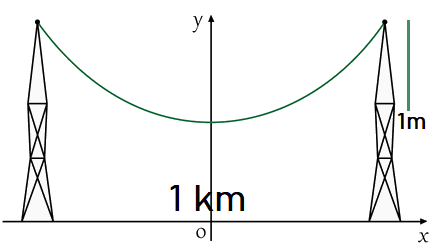
\includegraphics[width=0.3\textwidth]{catenary}
%    \end{figure*}
%
%    Solution is given by the equation
%    \[
%        \lambda \cdot \cosh\Bigl(\frac{500}{\lambda}\Bigr) - \lambda - 1 = 0
%    \]
%    Solve for $\lambda$, which can be used to compute the length of the cable
%    ($\lambda$ here is the radius of curvature at apex).
%    So, we want to find the root of this equation.
%    This is difficult to solve analytically, so we can find 
%    an approximation of $\lambda$.
%\end{example}

%\subsection{Bisection method}
%For cases like
%\begin{align*}
%    f(x) &= 12 x^2 - 5x - 2 = 0\\
%    &=(4x + 1)(3x - 2q)
%\end{align*}
%we can solve using the formula, and get $x_1 = -\frac{1}{4},\ x_2 = \frac{2}{3}$.
%But this does not work for a more complex problem, e.g.
%$f(x) = \log(3 + x^4) + 3\sin(x) = 0$.

%\begin{itemize}
%    \item {
%        We need to find an algorithm that gives a \textit{robust}
%        root localization (has to work for any nonlinear function).
%    }
%    \item {
%        We don't know how many roots there are. The algorithm should find at least one root per search.
%    }
%\end{itemize}
